% !TeX root = ../main.tex

\chapter{需求分析}

\section{系统概述}
容器化 CI/CD 流水线调度系统是一个自动化的工具,旨在提高软件开发的效率和速度。
它通过自动化编译、测试和部署过程,实现持续集成和持续交付。
该系统将支持敏捷开发的实践,通过自动化任务调度来优化研发团队的工作流程。
\section{需求导出}

首先,我们要明确我们的目标是设计一个高效、灵活且可靠的容器化CI/CD流水线调度系统。
该系统不仅要能够让用户根据自己的需求高度定制化自己的流水线,并提供稳定的执行,而且还要确保这一过程尽可能自动化,减少手动干预,提高开发效率和代码质量。
此外,系统还需要能够适应不断变化的开发需求,支持快速迭代,以满足敏捷开发的要求。

在了解了这些基本目标之后,我们通过与各个利益相关者的深入访谈,识别出了以下具体需求:

\paragraph{开发团队需求}
开发团队期望系统能提供一站式服务,自动完成从代码提交到部署的整个流程。
并且对系统的定制性有一定要求,开发团队希望流水线系统支持丰富的功能支持,以便满足多样化的需求。

\paragraph{测试团队需求}
测试团队希望流水线平台能够充分自动化,以缓解测试的人力资源需求,希望系统能够自动执行各种测试,包括单元测试、集成测试和性能测试等;
同时希望系统能够生成详细的测试报告,帮助测试人员快速发现和跟踪问题。

\paragraph{运维团队需求}
运维团队更加注重功能性和稳定性。运维团队希望系统支持庞大而复杂的流水线,以支持企业软件栈全面的集成与交付。
同时希望流水线能够支持一系列的人工操作,以便在流水线的执行过程中对流水线进行干预和把控。
稳定性方面,运维团队希望系统能够应对高峰期时的突发流量,并且出现异常时能快速恢复,以保证高可用性。

结合以上需求,我们希望能够设计出一个不仅功能强大,而且可用性强、稳定可靠的CI/CD流水线调度系统。

\section{功能性需求}

\subsection{术语描述}
为了清晰地描述系统需求,首先需要对CI/CD流水线中一些基本术语进行解释:

\paragraph{任务(Task)}
任务表示流水线中执行的一个单独的、不可再分的原子任务。
一个原子任务只完成一件事,如拉取Gitlab仓库代码、开源合规扫描、执行一个Shell脚本等。
任务必须包含在作业(Job) 内,同一个作业内的任务按顺序串行执行。

\paragraph{作业(Job)}
作业表示流水线中将要调度到执行器中执行的一系列原子任务的集合,是执行器执行的最小单位。
一个作业将运行在一个独立的运行环境中,它有以下特性:
\subparagraph{由多个任务组成;}
\subparagraph{作业内一个任务失败,则整个作业失败,其余任务将不会运行。}

\paragraph{阶段(Stage)}
阶段是一系列作业的逻辑集合。它的存在是为了更清晰的描述和管理流水线,它有以下特性:
\subparagraph{由多个作业组成;}
\subparagraph{同一个阶段下的不同作业执行方式为并行,当某个作业失败后,其它的作业会继续运行;}
\subparagraph{阶段内一个作业失败,则整个阶段失败。}

\paragraph{流水线(Pipeline)}
流水线是一个执行一系列作业的自动化工作流,它有以下特性:
\subparagraph{由多个阶段组成;}
\subparagraph{同一个流水线下的阶段串行执行,一个阶段失败,将不会执行后续阶段;}
\subparagraph{流水线内一个阶段失败,则该流水线失败。}

图~\ref{fig:流水线示意图}是图~\ref{fig:典型流水线示意图}的流水线按照以上概念进行的逻辑边界划分,它反映了流水线、流水线阶段、流水线作业和流水线任务的层级关系。
当该流水线被手动触发后则进入第一个阶段,该阶段包括两个作业——单元测试和静态代码检查,这两个作业将并行执行,在作业执行的过程中,每个作业内部的任务将顺序执行。
当这两个作业都成功后,流水线进入第二个阶段,再执行第二个阶段中的作业——编译并上传镜像。
以此类推,在没有人工干预的情况下,流水线将自动化地执行下去,直到某个作业执行失败则流水线失败,所有作业都执行成功则流水线成功。

\begin{figure}[h]
  \centering
  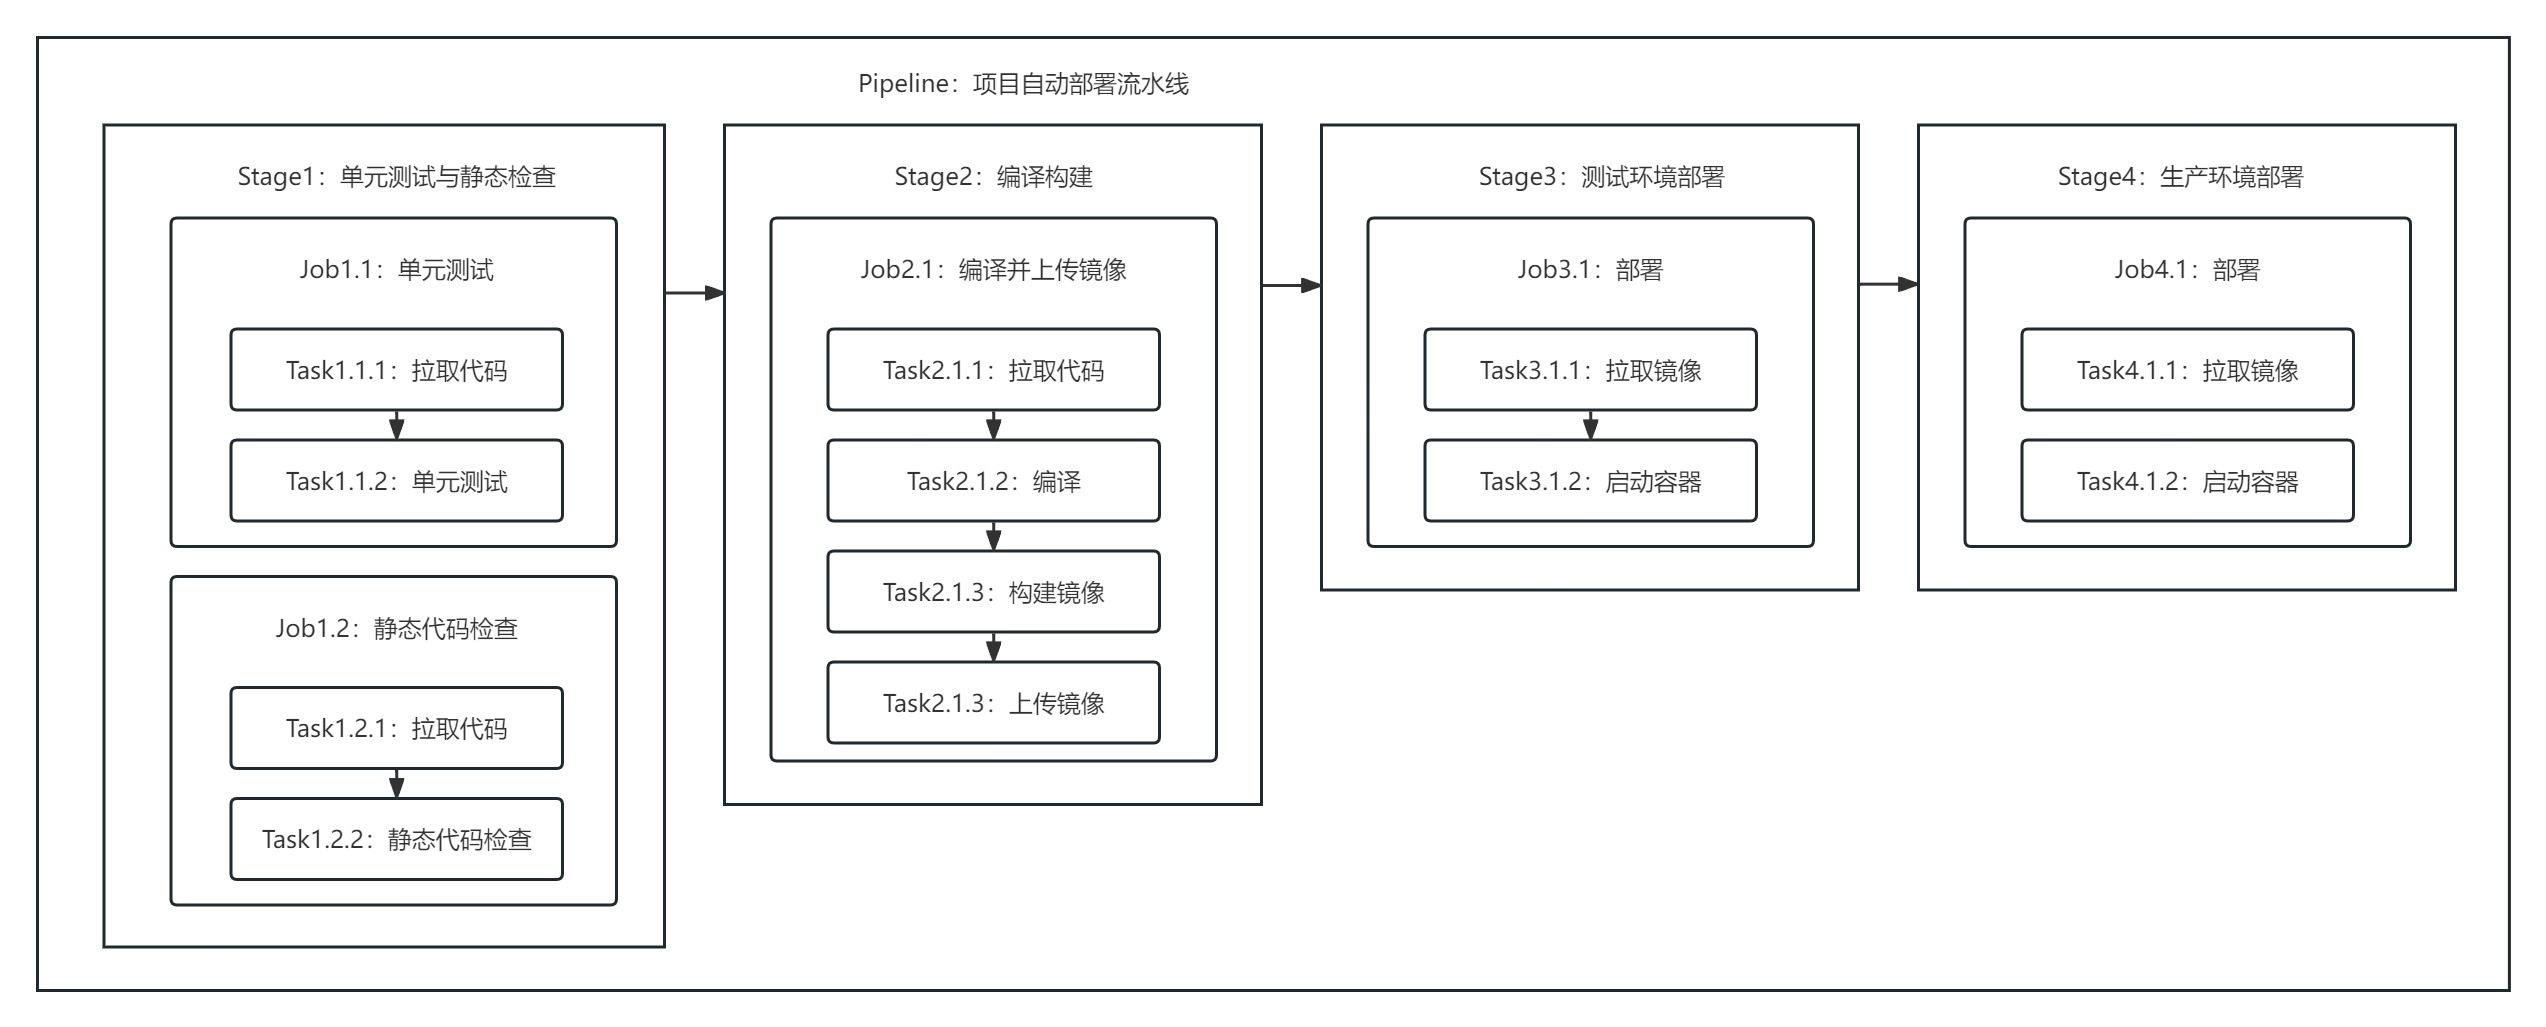
\includegraphics[width=1\textwidth]{流水线示意图.jpg}
  \caption{流水线示意图}
  \label{fig:流水线示意图}
\end{figure}

\subsection{流水线管理需求}
对于一个流水线系统来说,需要提供给用户对流水线进行增删改查的基本操作,主要包括:

\paragraph{创建并配置流水线}
CI/CD流水线的形态十分复杂,包含了三种不同类型的子概念:阶段、作业和任务,每个子概念中又有一系列的属性需要配置,如名称、触发类型等。
创建流水线时仅仅只创建流水线是无法运行的,流水线本质上只是对流程的抽象,对其中子概念的封装,所以创建流水线的同时必须同时进行一系列配置。

在创建流水线时,用户首先需要根据其业务需求,创建出不同的子概念,比如用户想要创建一个支持编译、测试和部署的流水线,用户则可以先按顺序创建出三个流水线阶段,
再在界面中通过拖拽等方式编排各个阶段的位置,以体现不同阶段的前后顺序,再在不同的阶段里创建一系列的作业,最后在已创建的作业里创建任务,至此完成了流水线结构的创建;
然后,用户需要进行流水线配置,也就是规定流水线中各个作业和任务都要做什么事情,系统应为每个用户已创建的子概念提供表单,以便用户为各个子概念填写配置信息。

总而言之,创建流水线时,系统需要提供给用户友好的交互页面,以便用户完成流水线结构的创建与配置填写。

\paragraph{编辑流水线配置}

系统应支持用户编辑已创建好的流水线,方便用户根据业务需求对流水线的结构和配置进行调整。

\paragraph{查看流水线配置及其运行记录}
系统提供友好的UI界面以便用户查看流水线配置。
同时,因为一条流水线能够被反复运行,所以一条流水线会产生多次运行记录,包括当次运行的各个子概念的最终状态、运行时间、日志等等,这些运行记录也应提供入口给用户查看。

\paragraph{删除流水线}
系统应支持用户删除不再使用的流水线。

流水线管理模块用例图如图~\ref{fig:流水线管理用例图}。

\begin{figure}[h]
  \centering
  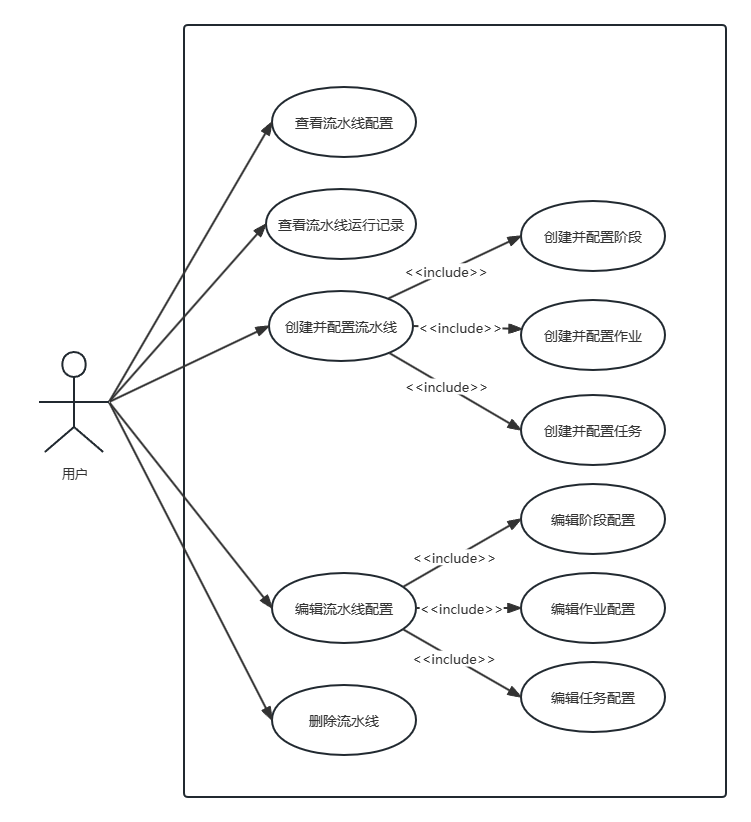
\includegraphics[width=0.8\textwidth]{流水线管理用例图.png}
  \caption{流水线管理用例图}
  \label{fig:流水线管理用例图}
\end{figure}


\subsection{人为干预需求}
当用户使用已经创建好的流水线的过程中,为满足用户对流水线的复杂操作需求,提高流水线的灵活度,CI/CD调度系统需要支持用户在流水线执行过程中主动对流水线的执行情况进行干预;
干预行为主要包括:

\paragraph{手动触发(Trigger)}
流水线的触发通常分为自动触发和手动触发两种方式

\paragraph{取消(Cancel)}
当用户在流水线的运行过程中,意识到流水线的后续执行会产生自己不期望的后果时,CI/CD调度系统应支持用户将其取消。
注意,当阶段或作业被取消后,系统应视为其已经失败,应阻止与其串行的后续阶段或作业的继续执行。

\paragraph{重试(Retry)}
流水线中某个作业的失败往往不是必现的,当用户认为某个失败的作业并非源于配置或者代码本身,而是因为运行环境、网络稳定性等因素导致失败时,CI/CD调度系统应支持用户将其重试。

\paragraph{跳过(Skip)}
通常来说,一条精心配置的流水线包含非常多的阶段和作业。但复用这条流水线的各个用户的需求可能各不相同。
当某个阶段或者作业用户认为没有必要执行,或者运行时间过长用户不希望再等待时,CI/CD调度系统应支持用户将其跳过。
注意,与“取消”操作相反,当阶段或作业被跳过后,系统应视为其已经成功,应立即继续与其串行的后续阶段或作业的继续执行。

\paragraph{人工审核(Review)}
当流水线运行到某个阶段或某个作业时,为确保后续按期望执行,并保证流水线产物的质量,CI/CD调度系统应支持用户在某个阶段或作业开始前,加入人工审核的环节。
同时,这一功能应支持流水线的编辑者自行设置审核人和审核的通过条件,比如设置了两位部门领导作为审核人,当任意一位审核人进入系统并点击“准入”后,该阶段或作业即开始执行;当两位审核人都点击“中止”后,该阶段或作业则被视为取消。

以上人工干预行为分别适用于一个或多个流水线中的子概念(流水线、阶段、作业和任务),依据对常见业务场景的分析,各个概念应支持的人工干预行为如表~\ref{tab:各个子概念应支持的人为干预行为表}:
\begin{table}[h]
  \centering
  \caption{各个子概念应支持的人为干预行为表}
  \label{tab:各个子概念应支持的人为干预行为表}
  \begin{tabular}{cl}
    \toprule
    子概念     & 人为干预行为                                     \\ 
    \midrule
    流水线     & 手动触发、取消 \\
    阶段       & 人工审核、取消、重试、仅重试阶段中失败作业   \\
    作业       & 手动触发、人工审核、取消、跳过、重试      \\
    任务       & 不允许人为干预       \\
    \bottomrule
  \end{tabular}
\end{table}

综上,得出流水线人为干预模块用例图如图~\ref{fig:流水线人工干预用例图}。

\begin{figure}[h]
  \centering
  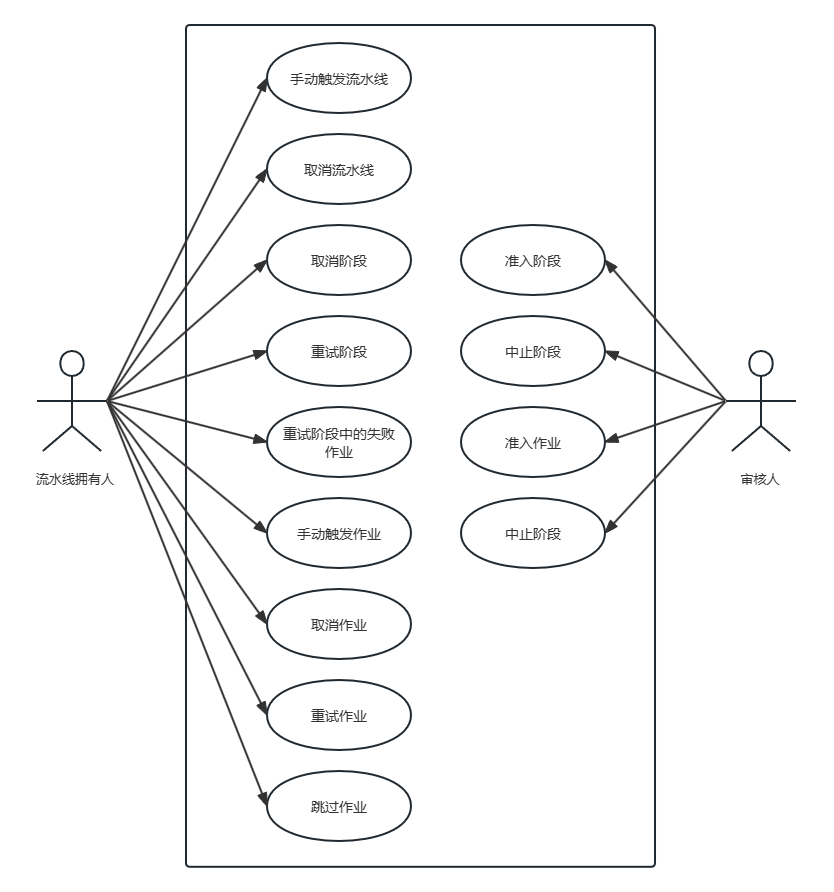
\includegraphics[width=0.8\textwidth]{流水线人工干预用例图.png}
  \caption{流水线人工干预用例图}
  \label{fig:流水线人工干预用例图}
\end{figure}

\subsection{状态流转需求}
在流水线的执行过程中,流水线中的每个子概念都在不同的状态间流转,通常来说应有如下状态:
就绪中(Pending)、执行中(Running)、执行成功(Success)、执行失败(Failed)、被跳过(Skipped)、被取消(Canceled)。
各个状态的具体解释如表~\ref{tab:状态解释表}。
\begin{table}[h]
  \centering
  \caption{状态解释表}
  \label{tab:状态解释表}
  \begin{tabular}{cl}
    \toprule
    状态           & 解释                                     \\
    \midrule
    就绪中         & 一切准备工作就绪,等待被自动执行、手动执行或审核通过\\
    执行中         & 正在被执行                 \\
    执行成功       & 顺利执行完毕后的状态        \\
    执行失败       & 执行过程中出错后的状态       \\
    被跳过         & 被用户人为干预执行“跳过”后的状态         \\
    被取消         & 被用户认为干预执行“取消”后的状态         \\
    \bottomrule
  \end{tabular}
\end{table}
以上状态适用于流水线中的各个子概念。

CI/CD调度系统需要保障流水线作业能够进行正确的状态流转,以保证用户能够正确、及时地得知流水线的执行情况。
同时,状态的正确流转也是流水线能按照正确逻辑链路执行的保证,系统需要结合当前流水线内各个子概念的状态,结合用户的人为操作,来判断流水线接下来的状态。
图~\ref{fig:流水线作业状态图}以作业为例,描述了其状态转移流程。

\begin{figure}[h]
  \centering
  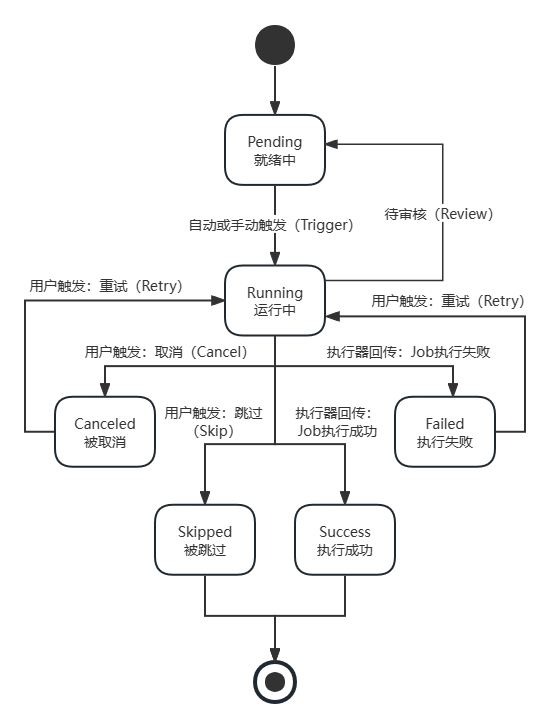
\includegraphics[width=0.8\textwidth]{流水线作业状态图.png}
  \caption{流水线作业状态图}
  \label{fig:流水线作业状态图}
\end{figure}


\subsection{自动触发需求}
自动化是CI/CD流水线提高软件团队研发效能的保证。通常来说,用户会希望某个指定仓库的代码出现变更的时候,CI/CD系统中的流水线便能自动触发。
系统能够某种感知或监听

\subsection{流水线作业合理调度需求}
\label{sec:流水线作业合理调度需求}

作业是流水线执行器中执行的最小单位,CI/CD调度器作为流水线配置与作业实际执行环境的中间环节,需要从作业排队、一致性分发、统一调度等方面保证作业的合理调度。

首先,系统需要保证作业的执行顺序与其被调度的顺序一致,即先来先执行。其次,当相当数量的作业被调度,超过了执行器的承载能力时,系统应能保证作业的阻塞等待,当前执行的作业结束执行后,再执行阻塞中的作业。
以上两点需求业内往往借助开源的消息队列服务实现,如RocketMQ等,借助消息队列先进先出和持久化的特性,保证了作业的调度顺序和阻塞等待。

然后,系统需要完成流水线作业的分配任务,将作业能够合理的分配给不同的作业执行模块。
当调度器判断应该调度某个作业时,CI/CD调度器将根据流水线配置时用户预填写的内容封装作业信息,再交付给执行器执行任务。
这一特性往往通过消息队列中消息的Tag和Title概念来实现对作业的精确分配。
同时,系统需要能够保证一个作业只能被一个执行器所执行,不能被多个执行器重复执行。


\section{非功能性需求}

除功能性需求外,系统需要满足以下非功能需求:

\paragraph{高性能}
本系统致力于提高效能,提升用户的研发效率,需要保证优秀的性能和较短的响应时间。
当用户进行流水线管理时,对流水线配置的增删改查应在1s内完成;
当用户人为干预流水线时,系统应在2s内给予用户反馈;
当流水线中阶段、作业或者任务的状态发生改变时,应在5s内对用户进行展示。

\paragraph{高稳定性}
CI/CD流水线系统的可靠性和稳定性尤为重要,一旦系统发生故障则直接影响整个企业的开发人员、测试人员和运维人员,阻塞代码合并、业务提测、系统发布等流程。
本系统可以借助以Kubernetes为代表的容器编排系统,实现横向扩展和故障转移的能力,以保证系统在使用高峰期时的稳定性。

\paragraph{高可用性}
CI/CD在当今的软件开发流程中是不可缺少的一环,系统应尽量保证7×24小时的服务提供。
依据业界常用指标,本系统需要至少达到99.99\%的可用性。
换算成服务时间则根据公式:服务可用率=成功调用数/总调用数,系统每一年的时间内,无法提供服务的总时间不能超过52分钟。

\paragraph{高易用性}
本系统应提供友好的交互逻辑,让缺乏相关知识背景的用户能够快速找到流水线的编辑与配置方式;
同时,由于CI/CD流水线通常有着复杂的层级与结构,系统应提供所见即所得的流水线拓扑结构界面,以便用户查看和调整;
最后,流水线的执行过程中应提供入口,将各个作业的运行日志可视化地展示给用户,方便用户时刻监控流水线作业的执行情况。

\paragraph{高安全性}
流水线一旦执行,可能会对其对应的系统产生影响,如发布新版本、发送通知等等。
为避免产生不期望的后果,系统应对流水线的触发以及各种操作进行严格的权限控制。
比如对某一条流水线的任何人为干预操作都应该由只能由流水线的归属人执行,其他人操作则提示无权限。
